\documentclass[UTF8,12pt]{article}
\usepackage{ctex}
\usepackage{indentfirst}
\usepackage{color}
\usepackage{hyperref}
\usepackage{graphicx}
\usepackage{subfigure}
\usepackage{pdfpages}
\usepackage{listings}
\hypersetup{
    hidelinks,
	colorlinks=true,
	allcolors=black,
	pdfstartview=Fit,
	breaklinks=true
}

\definecolor{dkgreen}{rgb}{0,0.6,0}
\definecolor{gray}{rgb}{0.5,0.5,0.5}
\definecolor{mauve}{rgb}{0.58,0,0.82}

\lstset{ %
  language=Octave,                % the language of the code
  basicstyle=\footnotesize,           % the size of the fonts that are used for the code
  numbers=left,                   % where to put the line-numbers
  numberstyle=\tiny\color{gray},  % the style that is used for the line-numbers
  stepnumber=2,                   % the step between two line-numbers. If it's 1, each line 
                                  % will be numbered
  numbersep=5pt,                  % how far the line-numbers are from the code
  backgroundcolor=\color{white},      % choose the background color. You must add \usepackage{color}
  showspaces=false,               % show spaces adding particular underscores
  showstringspaces=false,         % underline spaces within strings
  showtabs=false,                 % show tabs within strings adding particular underscores
  frame=single,                   % adds a frame around the code
  rulecolor=\color{black},        % if not set, the frame-color may be changed on line-breaks within not-black text (e.g. commens (green here))
  tabsize=2,                      % sets default tabsize to 2 spaces
  captionpos=b,                   % sets the caption-position to bottom
  breaklines=true,                % sets automatic line breaking
  breakatwhitespace=false,        % sets if automatic breaks should only happen at whitespace
  title=\lstname,                   % show the filename of files included with \lstinputlisting;
                                  % also try caption instead of title
  keywordstyle=\color{blue},          % keyword style
  commentstyle=\color{dkgreen},       % comment style
  stringstyle=\color{mauve},         % string literal style
  escapeinside={\%*}{*)},            % if you want to add LaTeX within your code
  morekeywords={*,...}               % if you want to add more keywords to the set
}


\setlength{\parindent}{2em}

\begin{document}

\begin{center}
    \tableofcontents
\end{center}
\newpage

\section{题目一}
\subsection{题目描述}
题目:给定一个英文ASCII码文件,统计文件中英文字母的频率,以十进制形式输出

基本要求:对于给定英文ASCII码文件,统计文件中每个英文字母的次数,计算的每个英文字母频率,以十进制形式输出每个英文字母对应的频率

\subsection{主要算法说明}
\subsubsection{磁盘调用}
在本实验中,需要能够读取文件。在汇编语言中,可以通过int 21h中断调用来实现。在本实验中,需要调用的是int 21h中断的3dh功能,即读取文件。其调用格式如下:

\begin{lstlisting}[title=中断调用,frame=shadowbox]
mov ah, 3dh
mov al, 0
mov dx, offset filename
int 21h
\end{lstlisting}

以上只是一般的文件调用,在本实验中,打开文件后还需要对文件进行各种操作,如读取文件、关闭文件等。因此从最开始的输入文件名开始分析。

\paragraph{输入文件名}
输入文件名需要在data区设置一个文件名字符串,用来接收用户输入的文件名,输入代码如下:

\begin{lstlisting}[title=输入文件名,frame=shadowbox]
    ;输入文件名
    lea dx,filename
    mov ah,0ah
    int 21h
\end{lstlisting}

\paragraph{对文件名进行操作并打开文件}
在这里对文件名进行操作,获取文件名的长度,然后再文件名后添加0,调用int 21h中断的3dh功能,打开文件。代码如下:

\begin{lstlisting}[title=对文件名进行操作并打开文件,frame=shadowbox]
    mov bl,filename+1;获取文件名长度
    mov bh,0
    mov [bx+filename+2],0;文件名后加0
    lea dx,filename+2
    mov ax,3d00h;打开文件
    int 21h
\end{lstlisting}

\paragraph{异常处理}
在文件打开过程中,可能会出现文件名输入错误造成无法打开的情况,因此需要对这种情况进行处理。在这里,如果文件打开失败,会返回一个错误代码,可以通过调用子过程实现。代码如下:

\begin{lstlisting}[title=异常处理,frame=shadowbox]
    jnc open
    mov si,offset error1;打开文件失败
    call dmess
    jmp continue
\end{lstlisting}

其中,dmess是一个子过程,用来输出错误信息,代码如下:

\begin{lstlisting}[title=dmess,frame=shadowbox]
    dmess proc
    dmess1:
        mov dl,[si]
        inc si
        or dl,dl
        jz dmess2
        mov ah,02h
        int 21h
        jmp dmess1
    dmess2:
        ret
    dmess endp
\end{lstlisting}

通过打印错误信息,可以让用户知道错误的原因,然后子过程结束,跳转到continue标签处,重新输入文件名。

\subsubsection{读取文件}
打开文件后,对文件进行读取,在这里调用readchar子过程进行单一字符的读取,然后调用punch子过程对字符出现频率进行统计,同时对读取异常进行处理;如果读取到文件尾部,则跳转typeok并打印读取到的字符串,代码如下:

\begin{lstlisting}[title=读取文件,frame=shadowbox]
    go:
    call readchar;读取一个字符
    jc readerror;读取失败
    cmp al,eof;判断是否到文件尾
    jz typeok;到文件尾,显示结果
    call punch;统计字符
    jmp go;继续读取
\end{lstlisting}

\paragraph{readchar子过程}
readchar子过程用来读取一个字符,调用int 21h中断的3fh功能,代码如下:

\begin{lstlisting}[title=readchar子过程,frame=shadowbox]
    readchar proc
        mov cx,1
        mov dx,offset buffer
        mov ah,3fh
        int 21h
        jc r1
        cmp ax,cx
        mov al,eof
        jb r2
        mov al,buffer

    r2:
        clc
    r1:
        ret
    readchar endp
\end{lstlisting}

其中,将读取到的字符存储在buffer中,如果读取失败,则返回一个进位标志,如果读取成功,则返回一个进位标志和一个零标志,如果读取到文件尾,则返回一个进位标志和一个负标志。

punch子过程对字符串进行计数,同时在技术之前会打印该字符,在后面将会单独展开。

\paragraph{异常处理}
读取字符时遭遇读取异常,调用dmess子过程返回错误信息,代码如下:

\begin{lstlisting}[title=异常处理,frame=shadowbox]
    readerror:
    mov si,offset error2
    call dmess
\end{lstlisting}

\paragraph{读取完成}
当读取到eof时,跳转到typeok标签处,关闭文件,然后打印统计到的结果,代码如下:

\begin{lstlisting}[title=读取完成,frame=shadowbox]
    typeok:
    mov ah,3eh;关闭文件
    int 21h
    mov dl,0ah
    mov ah,2
    int 21h
    call show
\end{lstlisting}

\subsubsection{统计字符}
统计字符是本实验中最核心的功能,需要对每个字符出现的次数进行统计以便后面的打印。在这里,使用了一个26个元素的数组来存储每个字符出现的次数,data段定义如下:

\begin{lstlisting}[title=定义数组,frame=shadowbox]
    array db 26 dup(0)
\end{lstlisting}

在统计字符前,先打印该字符,保留dx中原有值,需要将dx中的元素进栈,然后再打印该字符,代码如下:

\begin{lstlisting}[title=打印字符,frame=shadowbox]
    push dx
    mov dl,al
    mov ah,02h
    int 21h
    pop dx
\end{lstlisting}

在统计字符时,本实验采取的是不区分大小写,因此在判断的时候需要对大小写分别进行判断,采用ASCII码进行字符的判断,需要对字符的ASCII码区间进行划分,划分如下:

\begin{enumerate}
    \item 小写字母:97-122
    \item 大写字母:65-90
    \item 其他
\end{enumerate}

上述ASCII码值使用的是10进制,在进行比较的时候采用16进制。

\paragraph{第一轮比较}
在上述读取过程中,将读取到的字符存在了al中,将al中的元素存在ch中,然后将41h存在cl中,先进行一次比较,如果小于则跳转其他字符计数,实现代码如下:

\begin{lstlisting}[title=第一轮比较,frame=shadowbox]
    mov cl,41h
    lea di,array
    mov ch,al
    cmp ch,cl
    jb other
\end{lstlisting}

然后将ch中的值与5ah进行比较,如果大于则跳转higher2,准备进行第二轮比较,实现代码如下:

\begin{lstlisting}[title=第一轮比较,frame=shadowbox]
    cmp ch,5ah
    ja higher2
\end{lstlisting}

在确定了是大写字母后,进行字符的定位,如果cl、ch不匹配,则将cl++,再进行匹配,直到匹配成功,跳转char处进行计数,实现代码如下:

\begin{lstlisting}[title=第一轮比较,frame=shadowbox]
    h1:
    je char
    ja loop1

loop1:
    inc cl
    add di,1
    jmp h1
\end{lstlisting}

\paragraph{第二轮比较}
第二轮比较与第一轮比较类似,只是将41h改为61h,5ah改为7ah,实现小写字符的统计,实现代码如下:

\begin{lstlisting}[title=第二轮比较,frame=shadowbox]
    higher2:
    mov cl,61h
    lea di,array
    mov ch,al
    cmp ch,cl
    jb other
    cmp ch,7ah
    ja other

h2:
    cmp ch,cl
    je char
    ja loop2

loop2:
    inc cl
    add di,1
    jmp h2
\end{lstlisting}

\paragraph{其他字符}
如果不是大写字母和小写字母,则跳转到other标签处,实现代码如下:

\begin{lstlisting}[title=其他字符,frame=shadowbox]
    other:
    inc others
\end{lstlisting}

\paragraph{字符计数}
无论是大写字母还是小写字母,都会跳转到char标签处进行计数,采用记录偏移量的方式,将array的偏移量记录在di中,并将di中内容赋给ch来实现++,实现代码如下:

\begin{lstlisting}[title=字符计数,frame=shadowbox]
    char:
    sub ch,ch
    mov ch,[di]
    inc ch
    mov [di],ch
\end{lstlisting}

\subsubsection{打印结果}
在打印结果时,需要将结果转换为十进制,然后再打印。打印时按照顺序,并默认是大写输出,将array中的元素依次取出,并存在al中,通过调用display子过程进行十进制转化然后再打印,实现代码如下:

\begin{lstlisting}[title=打印结果,frame=shadowbox]
    show proc
        lea si,array
        mov di,41h
    loop3:
        lea dx,string1
        mov ah,09h
        int 21h
        mov dx,di
        mov ah,02h
        int 21h
        lea dx,string2
        mov ah,09h
        int 21h
        sub ax,ax
        mov al,[si]
        add si,1
        call display
        call endline
        inc di
        cmp di,5bh
        jb loop3
        ret
    show endp
\end{lstlisting}

\paragraph{display子过程}
display子过程用来将十进制转换为字符串,然后再打印,实现代码如下:

\begin{lstlisting}[title=display子过程,frame=shadowbox]
display proc near
    mov bl,10
    div bl
    push ax
    mov dl,al
    add dl,30h
    mov ah,02h
    int 21h
    pop ax
    mov dl,ah
    add dl,30h
    mov ah,02h
    int 21h
    mov dl,20h
    mov ah,02h
    int 21h
    ret
display endp
\end{lstlisting}

\paragraph{endline子过程}
endline用来调整打印的格式,实现代码如下:

\begin{lstlisting}[title=endline子过程,frame=shadowbox]
    endline proc near
    mov dl,20h
    mov ah,02h
    int 21h
    mov dl,20h
    mov ah,02h
    int 21h
    mov dl,20h
    mov ah,02h
    int 21h
    mov dl,20h
    mov ah,02h
    int 21h
    mov dl,20h
    mov ah,02h
    int 21h
    ret
endline endp
\end{lstlisting}

\subsection{运行界面的其他功能}
在本实验中,还加载了其他功能,如登录、统计询问、退出程序等功能,下面将对这些功能进行介绍。

\paragraph{登录}
在本实验中额外添加了登录过程,实现原理比较简单,在data段定义了一个用户名和密码,然后在程序开始时,进入登录界面,输入用户名和密码,如果正确则跳转到主界面,如果错误则跳转到登录失败界面,代码如下:

\begin{lstlisting}[title=登录,frame=shadowbox]
    input:        
    lea dx,username
    mov ah,09h
    int 21h
    
    lea dx,tempname
    mov ah,0ah
    int 21h
    
    cmp byte ptr tempname+1,05h
    jnz repeat1
    
    mov cx,5
    mov si,offset user
    mov di,offset tempname+2
    mov ax,datarea
    mov es,ax
    cld
    repe cmpsb
    jnz repeat1
    
    mov dx,offset tempname+2   ;显示输入的字符串
    mov byte ptr tempname[7],'$'
    call dosshow
    
    lea dx,password
    mov ah,09h
    int 21h
    
    lea dx,temppassword
    mov ah,0ah
    int 21h
    
    cmp byte ptr temppassword+1,06h
    jnz repeat2
    
    mov cx,6
    mov si,offset pass
    mov di,offset temppassword+2
    mov ax,datarea
    mov es,ax
    cld
    repe cmpsb
    jnz repeat2
    
    mov dx,offset temppassword+2
    mov byte ptr temppassword[8],'$'
    call dosshow
    
    jmp loginsuccess
\end{lstlisting}

\paragraph{统计询问}
在开始统计前,先进行询问,如果不需要统计则结束程序,如果需要统计则跳转到统计过程,代码如下:

\begin{lstlisting}[title=统计询问,frame=shadowbox]
    request:
        lea dx,starting;显示提示信息
        mov ah,09h
        int 21h

        mov ah,01h;获取键盘输入
        int 21h

        cmp al,'N';判断是否统计字符
        je finish;不统计字符,结束程序
        cmp al,'n'
        je finish

        cmp al,'Y';统计字符
        je continue
        cmp al,'y'
        je continue
		
		mov dl,0ah;回车换行
        mov ah,2
        int 21h
        mov dl,0dh
        mov ah,2
        int 21h

        jmp request;输入错误,重新输入
\end{lstlisting}

其中,continue标签处是统计过程,finish标签处是结束程序。

\subparagraph{continue标签}
在continue标签处,就提示输入文件名,然后调用打开文件过程,代码如下:

\begin{lstlisting}[title=continue标签,frame=shadowbox]
    continue:
		mov dl,0ah
        mov ah,2
        int 21h
        mov dl,0dh
        mov ah,2
        int 21h
		
        lea dx,string;显示提示信息
        mov ah,09h
        int 21h
        ...
\end{lstlisting}

\paragraph{finish标签}
在finish标签处,显示结束信息,然后调用4ch中断,结束程序,代码如下:

\begin{lstlisting}[title=finish标签,frame=shadowbox]
    finish:
        lea dx,ending;显示结束信息
        mov ah,09h
        int 21h
        mov ah,4ch;结束程序
        int 21h
\end{lstlisting}

\subsection{运行结果}
\subsubsection{起始界面}
\begin{figure}[htbp]
    \centering
    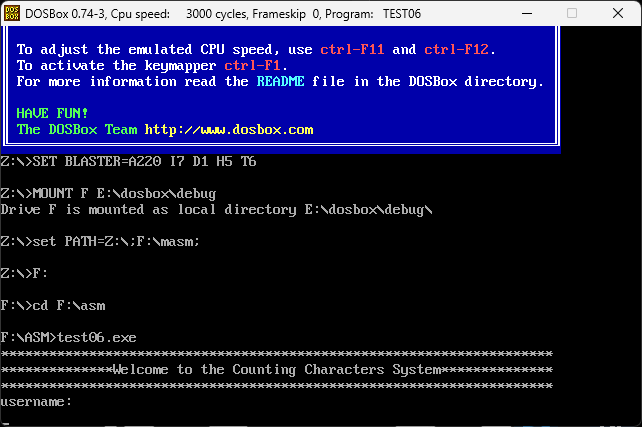
\includegraphics[width=0.8\textwidth]{img/1.png}
    \caption{起始界面}
\end{figure}

\newpage

\subsubsection{登录成功界面}
\begin{figure}[htbp]
    \centering
    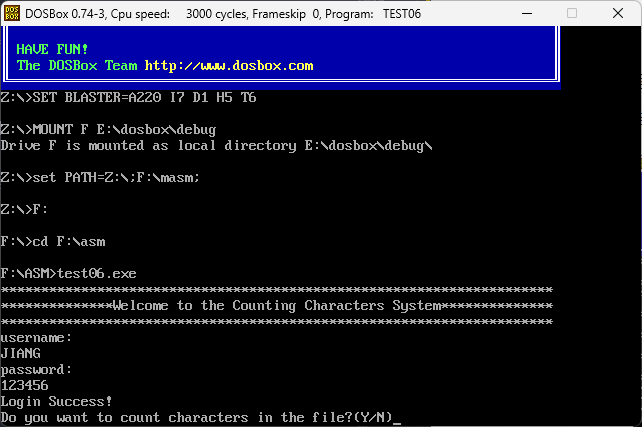
\includegraphics[width=0.60\textwidth]{img/2.png}
    \caption{登录成功界面}
\end{figure}

\subsubsection{登录失败界面}
\begin{figure}[htbp]
    \centering
    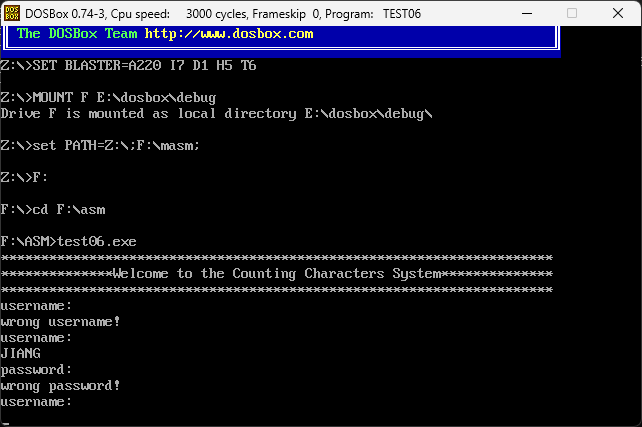
\includegraphics[width=0.60\textwidth]{img/3.png}
    \caption{登录失败界面}
\end{figure}

\newpage

\subsubsection{统计询问界面(Y)}
\begin{figure}[htbp]
    \centering
    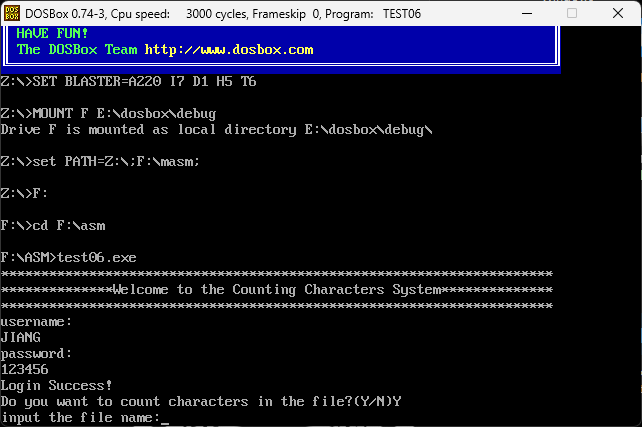
\includegraphics[width=0.60\textwidth]{img/4.png}
    \caption{统计询问界面(Y)}
\end{figure}

\subsubsection{统计询问界面(N)}
\begin{figure}[htbp]
    \centering
    
\includegraphics[width=0.60\textwidth]{img/5.png}
    \caption{统计询问界面(N)}
\end{figure}

\newpage

\subsubsection{文件输入与统计输出}
\begin{figure}[htbp]
    \centering
    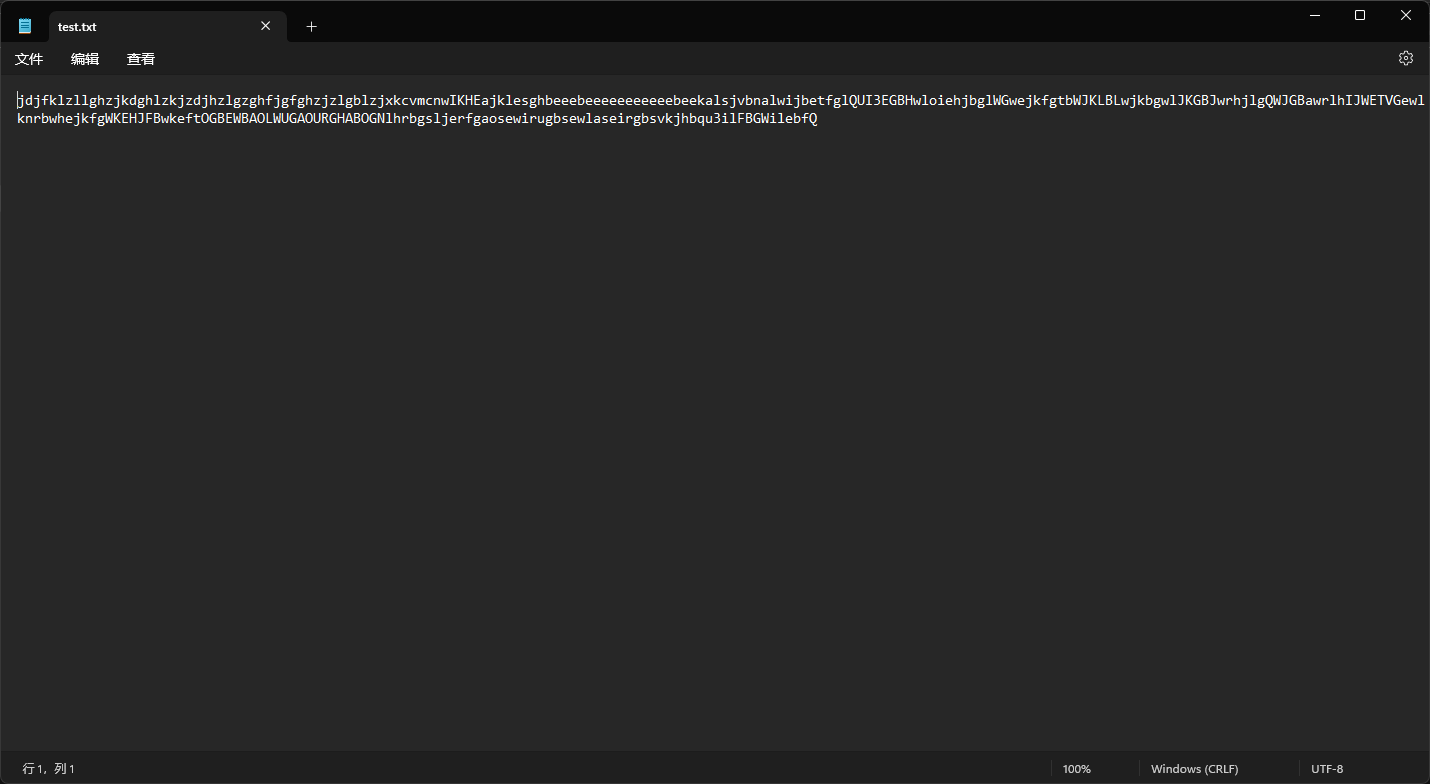
\includegraphics[width=0.64\textwidth]{img/8.png}
    \caption{待测文本}
\end{figure}

\begin{figure}[htbp]
    \centering
    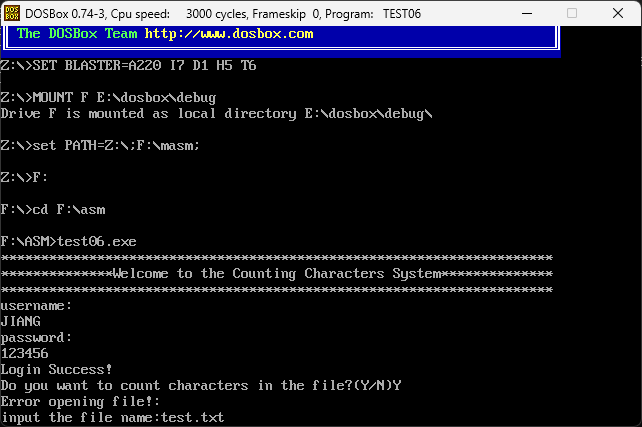
\includegraphics[width=0.64\textwidth]{img/6.png}
    \caption{文件输入}
\end{figure}

\newpage

\begin{figure}[htbp]
    \centering
    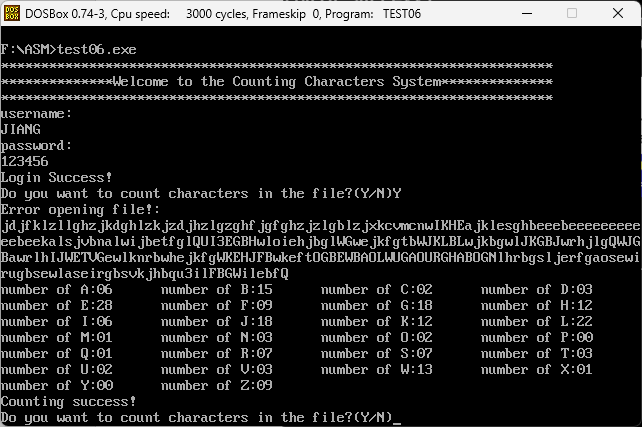
\includegraphics[width=0.64\textwidth]{img/7.png}
    \caption{统计输出}
\end{figure}

\subsubsection{文件名错误}
\begin{figure}[htbp]
    \centering
    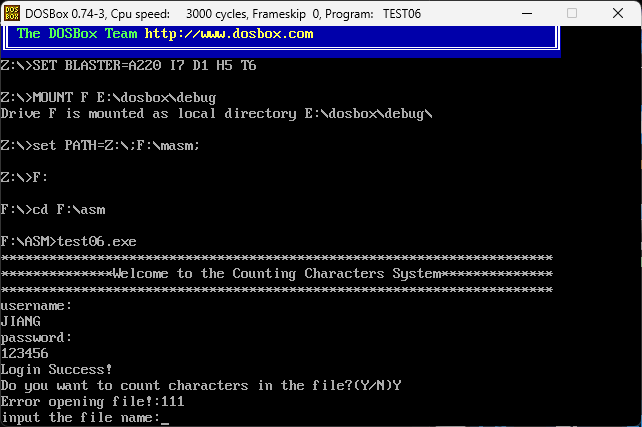
\includegraphics[width=0.64\textwidth]{img/9.png}
    \caption{文件名错误}
\end{figure}

\newpage

\subsection{课程设计总结}
\paragraph{问题与解决问题的过程}
\begin{enumerate}
    \item 对文件的操作不熟悉。在使用masm2015集成环境的时候,无论将文件放置在哪个安装目录下都无法打开文件,程序始终返回打开错误信息,然后选择使用dosbox手动编译、链接、打开程序,成功实现了对文件的操作
    \item 界面不够美观。在实验过程中,由于dosbox的年代比较久远,UI界面比较难优化,在调对齐的时候反复编译,最终使统计结果打印的比较整齐
\end{enumerate}

\paragraph{收获与感悟}
统计字符串的实验给我带来了以下收获:
\begin{itemize}
    \item 熟悉汇编语言:通过实验,我能够更加熟悉汇编语言的语法和基本指令。这对于理解计算机底层的工作原理非常重要,可以加深对计算机体系结构的理解。
    \item 理解字符编码:在统计英文字母频率的实验中,我需要对ASCII码进行处理。这让我更加深入地理解了字符编码的概念,以及不同编码方案对应的字符集。
    \item 掌握文件处理技巧:实验要求读取文件中的内容并统计英文字母的频率,这让我学会了在汇编语言中处理文件的基本技巧,包括打开文件、读取文件内容和关闭文件等。
    \item 提高问题解决能力:在实验过程中,我可能会遇到一些问题,例如文件读取失败、数据处理错误等。通过解决这些问题,我可以提高自己的问题解决能力和调试技巧。
    \item 培养耐心和细致:汇编语言编程需要非常细致和耐心,因为每个指令都需要仔细编写,并确保没有错误。通过实验,我可以培养这种耐心和细致的工作态度。
\end{itemize}

总的来说,通过完成这个汇编实验,我可以进一步加深对计算机底层的理解,学会处理文件和字符编码,并培养解决问题的能力和耐心。这些都对我未来的学习和职业发展有着积极的影响。

\subsection{参考文献}
《汇编语言程序设计》    雷向东,雷振阳,龙军   中南大学出版社

实验源码较长,因此将附录统一置于报告最后!

\newpage

\section{题目二}
\subsection{题目描述}
题目:用递归计算n!(n>=50), 以十进制数输出
基本要求:输入一个不小于50的整数n,用递归计算n!, 以十进制数输出

\subsection{主要算法说明}
在子程序嵌套的情况下,如果一个子程序调用的子程序就是它自身,这样的子程序称为递归子程序。求解N!本身是一个子程序,又因为N!=N*(N-1)!,所以求解N!的子程序可以调用求解(N-1)!的子程序,这样的子程序就是递归子程序。递归子程序的特点是:在子程序中调用自身,且每次调用时所用的参数不同。

递归通常使用堆栈来保存临时参数。递归调用展开时,保存在堆栈中的数据就有用:假设给定任意 n,即可计算 n-1 的阶乘。这样就可以不断减少 1,直到它等于 0 为止。根据定义,0!=l。而回溯到原始表达式 n! 的过程,就会累积每次的乘积,直到 n=0 为止。

\subsubsection{宏操作定义}
为了简化代码,同时减少提高代码的复用性,本实验中定义了一些宏操作。

\paragraph{OUTPUTCHAR}
为了能够输出字符,定义了一个宏操作,代码如下:

\begin{lstlisting}[title=OUTPUTCHAR,frame=shadowbox]
    ;字符输出
    OUTPUTCHAR MACRO AINCHAR	;将字符AINCHAR输出
        PUSH AX
        PUSH BX
        PUSH CX
        PUSH DX
            
        MOV DL,AINCHAR
        MOV AH,02H					;输出字符
        INT 21H
            
        POP DX
        POP CX
        POP BX
        POP AX
    ENDM
\end{lstlisting}

其中,对AX、BX、CX、DX进行了压栈操作,以便在输出字符后能够恢复原来的值,防止数据丢失

\paragraph{OUTPUTSTR}
OUTPUTSTR能够将一整个字符串输出,代码如下:

\begin{lstlisting}[title=OUTPUTSTR,frame=shadowbox]
    ;字符串输出
    OUTPUTSTR MACRO AIMSTR		;将字符串AIMSTR输出
        PUSH AX
        PUSH BX
        PUSH CX
        PUSH DX
            
        LEA DX,AIMSTR				;将AIMSTR的偏移地址送到DX寄存器
        MOV AH,09H					;09H字符串输出功能
        INT 21H
            
        POP DX
        POP CX
        POP BX
        POP AX
    ENDM
\end{lstlisting}

其中,对AX、BX、CX、DX进行了压栈操作,以便在输出字符串后能够恢复原来的值,防止数据丢失。

\paragraph{OUTPUTAX}
OUTPUTAX能够以十进制输出AX中的数值,代码如下:

\begin{lstlisting}[title=OUTPUTAX,frame=shadowbox]
    ;以10进制输出AX中的数值
OUTPUTAX MACRO				;将AX中的数值以10进制形式输出
	PUSH AX
	PUSH BX
	PUSH CX
	PUSH DX	
	CALL OUTPUTAXP			;调用进制输出过程	
	POP DX
	POP CX
	POP BX
	POP AX
ENDM
\end{lstlisting}

其中,通过调用COUTPUTAXP子过程实现十进制输出,代码如下:

\begin{lstlisting}[title=COUTPUTAXP,frame=shadowbox]
    OUTPUTAXP PROC
	MOV DX,0
	MOV CX,0						;用CX储存余数个数后续LOOP需要使用
	CMP AX,0						;判断AX中的值是否为0
	JNE	OUTPUTAXF1
	OUTPUTCHAR '0'
	JMP	OUTPUTAXPEXIT
		
OUTPUTAXF1:
	CMP AX,0						;判断AX中的值是否为0
	JE OUTPUTAXF2				;是则说明AX已经按位除完了
	MOV BX,10		   		 		;10进制
	DIV BX							;除10
	PUSH DX						;将余数入栈保存
	MOV DX,0
	INC CX							;计数循环取得的余数个数
	JMP OUTPUTAXF1
		
OUTPUTAXF2:						;循环输出取得的余数
	POP AX
	ADD AL,30H
	OUTPUTCHAR AL
    LOOP OUTPUTAXF2
OUTPUTAXPEXIT:  RET	
OUTPUTAXP	ENDP
\end{lstlisting}

\paragraph{OUTPUTNUM}
OUTPUTNUM能够将数字字符串AIMNUM表示的数值输出,代码如下:

\begin{lstlisting}[title=OUTPUTNUM,frame=shadowbox]
    ;输出字符串AIMNUM所表示的数值
    OUTPUTNUM MACRO AIMNUM
        PUSH AX
        PUSH BX
        PUSH CX
        PUSH DX
        PUSH SI
            
        LEA	BX,AIMNUM;用BX存储字符串AIMNUM在DS中的首地址	
        CALL OUTPUTNUMP	;调用字符串AIMNUM数值输出过程
            
        POP SI
        POP DX
        POP CX
        POP BX
        POP AX
    ENDM
\end{lstlisting}

其中,通过调用OUTPUTNUMP子过程实现字符串数值输出,代码如下:

\begin{lstlisting}[title=OUTPUTNUMP,frame=shadowbox]
    OUTPUTNUMP	PROC
OUTPUTNUMF1:
	MOV SI,-2
OUTPUTNUMEND:					;使SI指向ANS的数值结尾处
	ADD SI,2
	MOV AX,[BX+SI]				;测试AX是否为-1
	CMP AX,-1
	JNE	OUTPUTNUMEND			;直到搜索到最后结尾-1
	
	SUB SI,2
	CMP SI,-2
	JE	OUTPUTNUMEXIT			;若为-2则说明ANS中不存在数据
	MOV AX,[BX+SI]				;取出ANS中的第一个数值到AX中 从低到高
	OUTPUTAX					;将AX中的数以10进制形式输出 是最高位不需要填0
	
OUTPUTNUMNEXT:	
	SUB SI,2
	CMP SI,-2
	JE	OUTPUTNUMEXIT
	MOV AX,[BX+SI]				;取出ANS中的数值到AX中 开始判断有多少0需要填充
	CMP AX,1000
	JAE	OUTPUTNUMF2			;AX中的数值大于等于1000时跳转
	OUTPUTCHAR '0'				;AX小于1000时先输出一个字符'0'
	CMP AX,100
	JAE	OUTPUTNUMF2
	OUTPUTCHAR '0'				;AX小于100时再输出一个字符'0'
	CMP AX,10
	JAE	OUTPUTNUMF2
	OUTPUTCHAR '0'				;AX小于10时再输出一个字符'0'

OUTPUTNUMF2:	
	OUTPUTAX					;将AX中的数以10进制形式输出
	JMP OUTPUTNUMNEXT		;跳转进行下一位数值的输出	
OUTPUTNUMEXIT:		
	RET	
OUTPUTNUMP	ENDP
\end{lstlisting}

\subsubsection{n值的输入}
在本实验中,采用int 21h中断的1号功能来实现n值的输入,字符默认输入到AL中,对输入进行判断,如果键入回车,则输入结束,如果键入数字,则将键入的数字ascii码减去30h,然后乘以10,再加上原来的值,实现代码如下:

\begin{lstlisting}[title=n值的输入,frame=shadowbox]
    TYPEIN:  ;输入需要求解的n值
    PUSH AX
    MOV AH,01H
	INT 21H					    ;字符默认输入到AL中
	CMP AL,13
	JE	TYPEINEXIT			    ;检测到回车后跳转AX的输出
	SUB	AL,48				    ;将字符转化为对应的数值
	MOV BH,0
	MOV BL,AL
	POP	AX		
	CMP AX,0				;当AX中的数值为0时,跳过乘法操作
	JE	TYPEINADD
	MOV CX,10
	MUL CX					    ;乘以10
TYPEINADD:
    ADD AX,BX
	JMP TYPEIN		
TYPEINEXIT:	
    POP AX						;将计算得到的数值出栈到AX中		
	POP DX
	POP CX
	POP BX
	MOV CX,AX					;求阶乘的数转至CX中
\end{lstlisting}

其中,将输入的字符转换为数字,每次输入一位数字,已知“0”的ASCII码为30h,因此将输入的字符减去30h,即可得到对应的数字。

\subsubsection{阶乘的计算}
阶乘的计算是本实验中最重要的部分,在前期处理中,已经得到了需要计算的n值并存储在AX中,接下来就是阶乘的计算。

\paragraph{阶乘结果寄存器的定义}
题目要求阶乘的数是不小于50的,根据8086的参数可知,单一寄存器都是16位的,因此单一寄存器最大存储的数就是65535,根据简单的计算得到:8!=40320,9!=362880,因此不可能使用单一寄存器或者多寄存器来存储阶乘的结果,因此需要定义单独的结果存储变量来存放阶乘结果,定义如下:

\begin{lstlisting}[title=阶乘结果寄存器定义,frame=shadowbox]
    ANS	DW	1,3000 DUP(-1)			;储存运算结果 存入一个1应对输入0的情况
    ANSH	DW	3000 DUP(0)			;相对高位
    ANSL	DW	3000 DUP(0)			;相对低位
\end{lstlisting}

其中,ANS是结果存储变量,每一个单元能存放四位数,ANSH和ANSL在程序中的作用如下:将ANS中的数值与10000进行比较,如果小于10000,则直接存储在ANS的单元中;如果大于10000,则将该数除以10000,商存于ANSH中,余数存于ANSL中。

\begin{lstlisting}[title=数乘,frame=shadowbox]
    MOV BX,1						;BX逐步求阶的乘数
SAVENEXT:
	CMP CX,0
	JE	OUTPUTANS				;当CX中的值为0时,输出ANS中的数值
	PUSH CX					
	MOV SI,0						;SI指向ANS的起始位置
	
MULANS:					;对ANS中的所有数值进行乘BX操作,乘积大于等于10000的部分存储到ANSH中,小于10000的部分存储到ANSL中
	MOV AX,ANS[SI]		;取出ANS中的数值到AX中
	CMP AX,-1
	JE	TRANSFORM				;直到取得的数值为-1时,跳转
	MUL BX						;进行乘法操作
	
	PUSH CX	
	MOV CX,10000
	DIV CX							;除法操作 除以10000
	POP CX
		 
	MOV ANSL[SI],DX		    	;将余数存储到ANSL中			
	ADD SI,2
	MOV ANSH[SI],AX		    	;将商存储到ANSH中
	
	JMP	MULANS
\end{lstlisting}

然后对ANSL、ANSH的格式进行调整,将商调整到ANS的高位中,并将余数放回ANS的原位

\begin{lstlisting}[title=格式调整,frame=shadowbox]
    TRANSFORM:						;对ANS乘以BX得到的数值字符串ANSL和ANSH,进行格式调整,并将调整后的结果存储到ANS中去
	PUSH BX						;BX中的乘数入栈保存	
	MOV BX,0
	MOV SI,2
	
TRANSFORMF1:
	MOV AX,ANS[BX]				;取出ANS中的数值到AX中
	CMP AX,-1
	JE	TRANSFORMF2			;当ANS中的数值取完时,跳转
	
	MOV AX,ANSH[BX]		    ;取商到AX中
	ADD AX,ANSL[BX]		   	;加上此时所在位置对应的余数
	
	CMP AX,10000					;判断AX中的数值是否大于10000
	JB SAVEINTOANS				;小于10000时直接将数值存储到ANS中
	MOV DX,0						;大于10000时,将大于等于10000的部分存到高位的进位中去,小于10000的部分存储到ANS中
	PUSH CX
	MOV CX,10000
	DIV CX
	POP	CX
	MOV ANS[BX],DX				;小于10000的余数部分存储到ANS中
	ADD ANSH[SI],AX				;大于10000的高位部分添加到高位的进位中去
	
	ADD BX,2						;指针后移指向下一个数值
	ADD SI,2
	JMP	TRANSFORMF1
	
SAVEINTOANS:	
	MOV ANS[BX],AX				;将数值存储到ANS中
	ADD BX,2						;指针后移指向下一个数值
	ADD SI,2
	JMP	TRANSFORMF1
	
TRANSFORMF2:
	MOV AX,ANSH[BX]			;取出上一个商到AX中
	CMP AX,0
	JE	TRANSFORMF3			;若AX中的数值为0时 跳过下一步
	MOV ANS[BX],AX				;将上一位的商添加到ANS中
TRANSFORMF3:
	POP	BX						;BX中的数值出栈
	INC BX
	POP CX
	LOOP SAVENEXT
\end{lstlisting}

其中,对于不同的情况进行不同的调整,如果乘积小于10000,则直接存储到ANS中;如果乘积大于10000,则将乘积除以10000,商存于ANSH中,余数存于ANSL中,然后将ANSH中的数值添加到ANS的高位中,将ANSL中的数值存于ANS的原位中。

\subsubsection{阶乘结果的输出}
阶乘的结果存储在ANS中,调用OUTPUTNUM宏操作,将ANS中的数值输出,实现代码如下:

\begin{lstlisting}[title=阶乘结果的输出,frame=shadowbox]
    OUTPUTANS:						;输出数值字符串所表示的数值
	OUTPUTNUM ANS
\end{lstlisting}

\newpage

\subsection{运行界面}
\subsubsection{起始界面}
\begin{figure}[htbp]
    \centering
    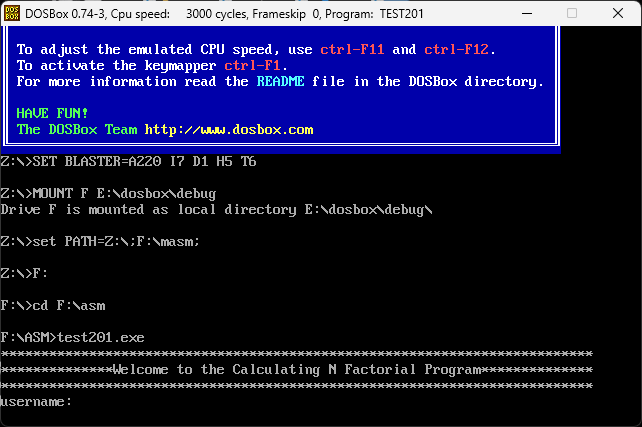
\includegraphics[width=0.6\textwidth]{img/10.png}
    \caption{起始界面}
\end{figure}

\subsubsection{登录成功}
\begin{figure}[htbp]
    \centering
    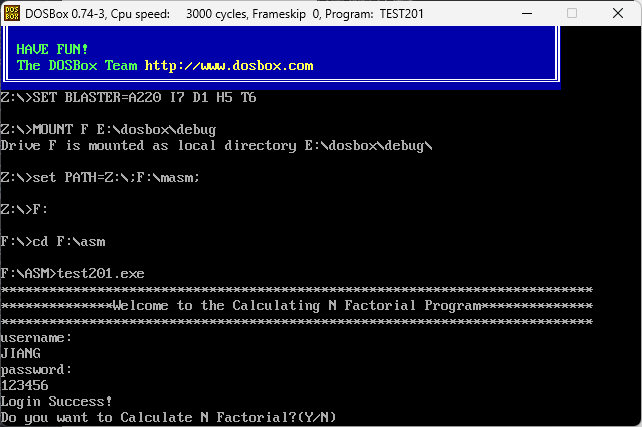
\includegraphics[width=0.6\textwidth]{img/11.png}
    \caption{登录成功}
\end{figure}

\newpage

\subsubsection{n值输入并计算}
\begin{figure}[htbp]
    \centering
    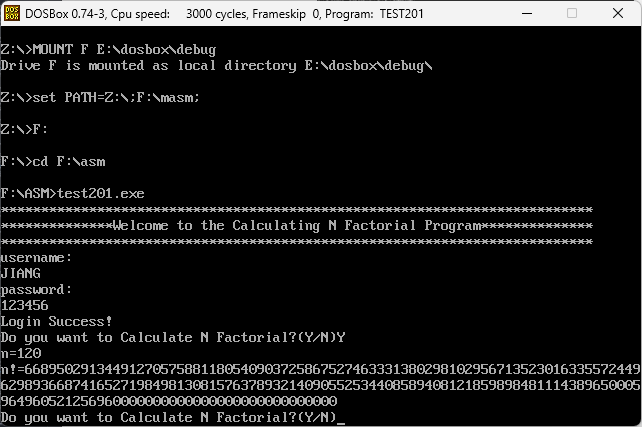
\includegraphics[width=0.6\textwidth]{img/12.png}
    \caption{n值输入并计算}
\end{figure}

\subsubsection{退出程序}
\begin{figure}[htbp]
    \centering
    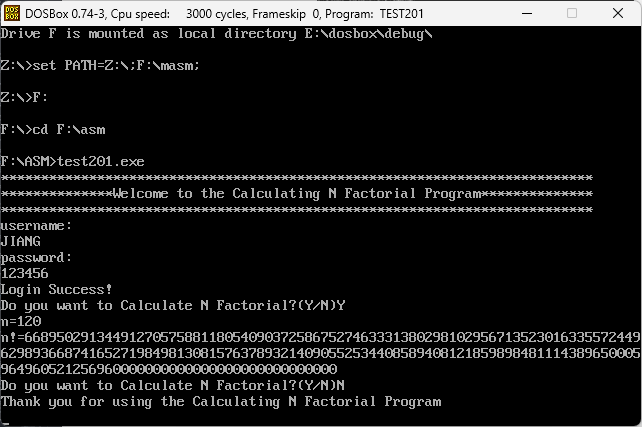
\includegraphics[width=0.6\textwidth]{img/13.png}
    \caption{退出程序}
\end{figure}

\newpage

\subsection{课程设计总结}
\paragraph{问题与解决问题的过程}
\begin{enumerate}
    \item 递归计算阶乘不熟悉:在开始编写代码时,对递归计算阶乘不熟悉,因此在编写代码时,出现了很多错误,例如:没有考虑到阶乘的结果超过16位的情况,没有考虑到阶乘的结果为0的情况等,通过不断的调试,最终解决了这些问题。
    \item 大数据的存储方式的改变:在开始编写代码时,我将阶乘的结果存储在一个单一的变量中,但是后来发现,单一的变量无法存储阶乘的结果,因此需要改变存储方式,将阶乘的结果存储在一个数组中,通过数组的方式来存储阶乘的结果。
\end{enumerate}

\paragraph{收获与感悟}
通过这次的汇编课设,我发现了自己在知识掌握和实践方面存在许多不足。首先,我的知识掌握不够扎实;其次,我在实践方面缺乏经验,这导致了很多错误的发生。在开始搭建大致框架后,我逐渐进行修改,最终成功地实现了目标。在实际运行过程中,遇到了多个问题和报错,但我能够及时解决这些问题。当遇到不懂的情况时,我会上网查阅相关知识。通过不断地经历错误和解决问题,我的能力得到了很大的提升,对知识的掌握也得到了巩固和强化,同时培养了分析和解决问题的能力以及独立思考的能力。因此,这次的汇编课设给我带来了很多收获。在汇编过程中,我使用了递归调用子程序的算法,这次经历使我对这些算法思想有了更清晰的理解。通过反复练习、总结和学习命令操作,我对汇编语言有了更深入的学习。

\subsection{参考文献}
《汇编语言程序设计》    雷向东,雷振阳,龙军   中南大学出版社

实验源码较长,因此将附录统一置于报告最后!


\section{题目三}
\subsection{题目描述}
题目:存储器系统设计

基本要求:设计一个存储器系统,包括存储器的地址空间、存储单元的位数、存储单元的个数、存储器的容量、存储器的读写功能、存储器的读写速度、存储器的结构、存储器的接口等。

\subsection{实验原理}
在微机系统中,常用的静态RAM 有6116、6264、62256等。在本实验中使用的是6116。6116 为2K*8位的静态RAM,其逻辑如图所示:

\begin{figure}[htbp]
    \centering
    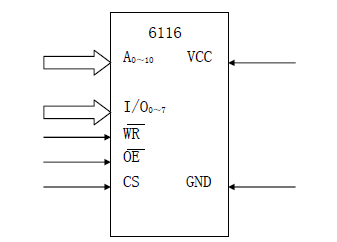
\includegraphics[width=0.8\textwidth]{img/14.png}
    \caption{6116逻辑图}
\end{figure}

其中A0~10 为11根地址线,I/O为0-7共8根数据线,CS为片选端,OE 为数据输出选通端,WR为写信号端。6116的工作方式如下表:

\begin{table}[htbp]
    \centering
    \caption{6116工作方式}
    \begin{tabular}{|c|c|c|c|c|}
        \hline
        控制信号 & CS & OE & WR & 数据线  \\
        \hline
        读 & 0 & 0 & 1 & 输入 \\
        \hline
        写 & 0 & X & 0 & 输出 \\
        \hline
        非选 & 1 & X & X & 高阻态 \\
        \hline
    \end{tabular}
\end{table}

实验所用的半导体静态存储器电路原理如图所示,实验中的静态存储器一片6116(2K×8)构成,其数据线接至数据总线,地址线由地址锁存器(74LS273)给出。地址灯AD0—AD7 与地址线相连,显示地址线内容。数据开关经一三态门(74LS245)连至数据总线,分时给出地址和数据。

\begin{figure}[htbp]
    \centering
    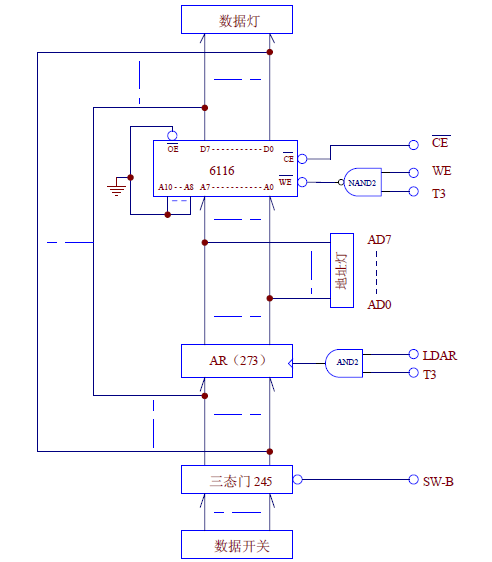
\includegraphics[width=0.6\textwidth]{img/15.png}
    \caption{半导体静态存储器电路原理图}
\end{figure}

因地址寄存器为8位,接入6116的地址A7—A0,而高三位A8—A10接地,所以其实际容量为256字节。6116有三个控制线:CE(片选线)、OE(读线)、WE(写线)。当片选有效(CE=0)时,OE=0时进行读操作,WE=0 时进行写操作。本实验中将OE常接地,在此情况下,当CE=0、WE=0 时进行读操作,CE=0、WE=1时进行写操作,其写时间与T3 脉冲宽度一致。控制信号SW-B为低电平有效,控制信号LDAR为高电平有效。

\subsection{实验步骤}
\subsubsection{选择实验器材}
根据实验原理图,将所需要的组件从组件列表中拖到实验设计流程栏中。

\subsubsection{搭建实验电路}
将已选择的组件进行连线(鼠标从一个引脚的端点拖动到另一组件的引脚端,即完成连线)。搭建好的实验如图所示:

\begin{figure}[htbp]
    \centering
    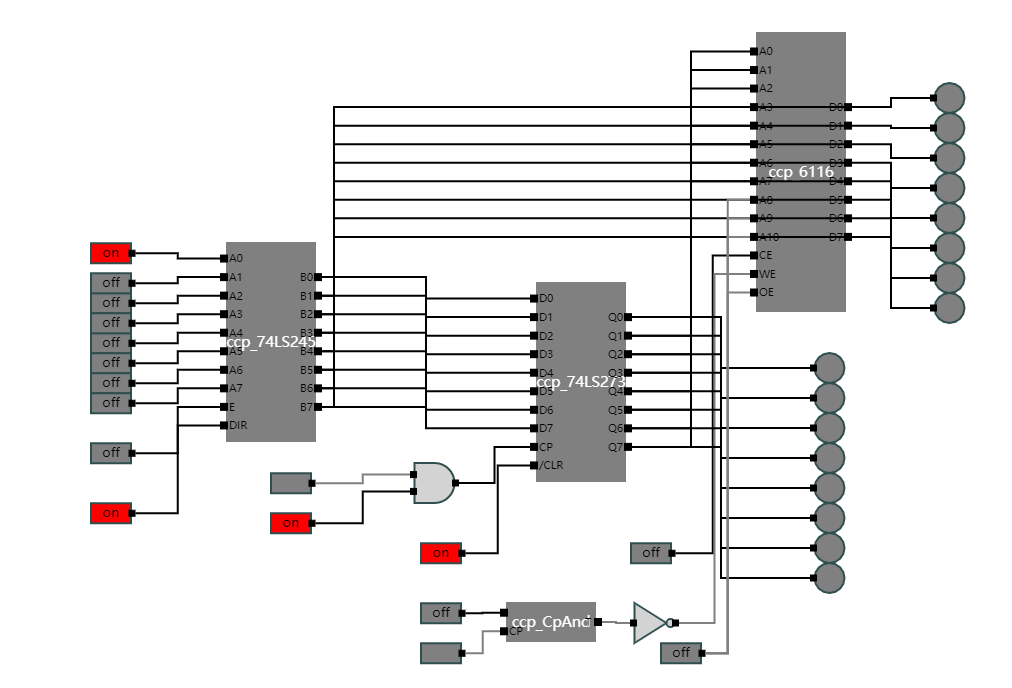
\includegraphics[width=0.9\textwidth]{img/19.png}
    \caption{实验电路}
\end{figure}

\subsubsection{初始化各芯片的控制信号}
初始化各芯片的控制信号,仔细检查无误后点击【电源开/关】按钮接通电源。

\subsubsection{写存储器}
给存储器的00、01、02、03、04地址单元中分别写入数据11H、12 H、13 H、14 H、15 H。

由存储器实验原理图看出,由于数据和地址全由一个数据开关给出,因此要分时地给出。下面的写存储器要分两个步骤,第一步写地址,先关掉存储器的片选(CE=1),打开地址锁存器门控信号(LDAR=1),打开数据开关三态门(SW-B=0),由开关给出要写入的存储单元的地址,双击单脉冲产生T3 脉冲将地址输入到地址锁存器;第二步写数据,关掉地址锁存器门控信号(LDAR=0),打开存储器片选,使之处于写状态(CE=0,WE=1),由开关给出此单元要写入的数据,,双击单脉冲产生T3 脉冲将数据写入到当前的地址单元中。写其他单元依次循环上述步骤。

写存储器流程如图所示(以向00号单元写入11H为例)。

\begin{figure}[htbp]
    \centering
    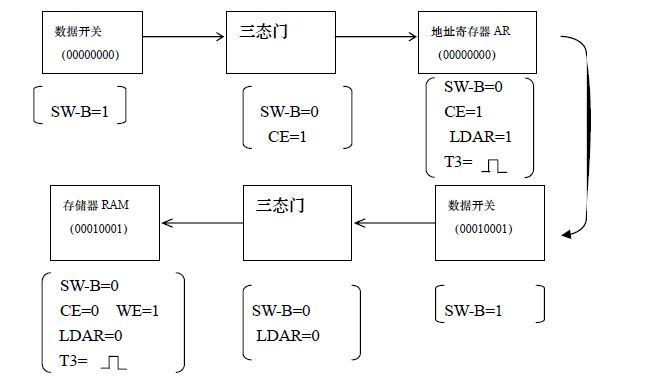
\includegraphics[width=0.8\textwidth]{img/17.png}
    \caption{写存储器流程}
\end{figure}

\subsubsection{读存储器}
依次读出第00、01、02、03、04号单元中的内容,观察上述各单元中的内容是否与前面写入的一致。同写操作类似,读每个单元也需要两步,第一步写地址,先关掉存储器的片选(CE=1),打开地址锁存器门控信号(LDAR=1),打开数据开关三态门(SW-B=0),由开关给出要写存储单元的地址,双击单脉冲产生T3 脉冲将地址输入到地址锁存器;第二步读存储器,关掉地址锁存器门控信号(LDAR=0),关掉数据开关三态门(SW-B=1),片选存储器,使它处于读状态(CE=0,WE=0),此时数据总线上显示的数据即为从存储器当前地址中读出的数据内容。读其他单元依次循环上述步骤。

读存储器操作流程如图所示(以从00 号单元读出11H 数据为例)

\begin{figure}[htbp]
    \centering
    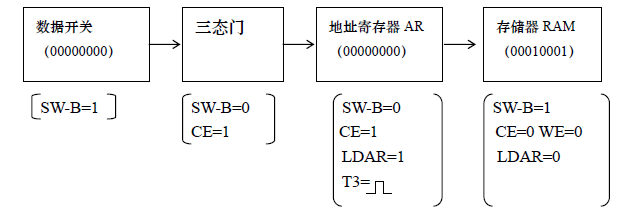
\includegraphics[width=1.0\textwidth]{img/18.png}
    \caption{读存储器流程}
\end{figure}

\newpage

\subsection{运行界面}


\subsection{课程设计总结}
通过本次实验,我获得了以下几方面的心得体会:

首先,我对逻辑器件的组成结构有了更深入的了解。实验使我熟悉了一些逻辑器件的工作原理,并验证了它们的组合功能。通过亲自动手进行实验,我更好地理解了逻辑器件的构成和功能。

其次,我学会了总线和各个器件之间的工作过程。在实验中,我了解了总线在连接各个器件时的重要作用,以及它们之间的数据传输过程。这让我对整个系统的运作有了更清晰的认识。

同时,实验中遇到了一些问题,但我成功地解决了它们。这个过程让我对所学知识更加牢固,提高了自己解决问题的能力。我也意识到在实验连线时需要细心,并且在操作过程中出现问题时,要能够快速检查并解决,以确保实验顺利进行。

这次实验是在虚拟平台上进行的,我遇到了灯泡不亮的问题,导致我不确定实验是否成功。我及时向老师反映了问题。这次经历让我明白了沟通与求助的重要性。另外,在连接各个器件时,我也注意到了注重美观和整洁的连接方式。

综上所述,通过本次实验,我对逻辑器件的组成和工作原理有了更深入的了解,掌握了可靠的静态存储器的工作特性和使用方法。我通过解决问题提高了自己的知识储备,并且意识到了良好的沟通和整洁的实验操作对于实验成功的重要性。

\subsection{参考文献}
《计算机组成原理(第二版)》  唐朔飞,李国杰,李国杰   清华大学出版社

\newpage

\section{题目四}
\subsection{题目描述}
题目:乘法器设计

基本要求:学习乘法器结构,逻辑控制单元设计方法,提出设计方案,小组讨论研究,实现设计方案。

\subsection{实验原理}
两位二进制数乘法器是一种简单的数字电路设计,用于执行两个二进制数的乘法运算。下面是一个基本的两位二进制数乘法器的设计:

\begin{enumerate}
    \item 输入:设计一个两位二进制数乘法器,需要两个两位二进制数作为输入。假设这两个数分别为A和B。
    \item 乘法运算:将A的每一位与B的每一位相乘,得到四个部分乘积。对于两位数的乘法,共有四个部分乘积需要计算。
    \item 部分乘积对齐:对于第i个部分乘积,将其左移i位,以对齐相应的位数。
    \item 部分乘积相加:将所有四个部分乘积相加,得到最终的乘积结果。
    \item 结果输出:输出最终的乘积结果,其位数为输入位数的两倍。
\end{enumerate}

以下是一个具体的示例,展示了两位二进制数乘法器的设计过程:

输入:A = a1a0, B = b1b0

\begin{enumerate}
    \item 计算部分乘积:\\ P0 = a0 * b0\\ P1 = a0 * b1\\ P2 = a1 * b0\\ P3 = a1 * b1
    \item 对齐部分乘积:\\ P0 = P0 << 0 (不需要对齐)\\ P1 = P1 << 1 (左移1位)\\ P2 = P2 << 1 (左移1位)\\ P3 = P3 << 2 (左移2位)
    \item 相加部分乘积:\\ Result = P0 + P1 + P2 + P3
    \item 结果输出:\\ 输出Result作为两位二进制数的乘积结果。
\end{enumerate}

需要注意的是,这只是一个基本的两位二进制数乘法器的设计示例。在实际应用中,可能需要考虑更多的优化和细节,如进位处理、结果截断、错误处理等。此外,也可以使用更复杂的乘法器结构来提高性能和效率。

\newpage

\subsection{实验设计}
实验中采用两块74LS138芯片,其中一位数值进行片选信号,每一块芯片各自表示8个数值,因此可以表示16个数值,在数电设计中,列出真值表就可以确定逻辑电路的设计,如下表所示:

\begin{table}[htbp]
    \centering
    \caption{74LS138芯片真值表}
    \begin{tabular}{|c|c|c|c|c|c|c|c|}
        \hline
        A1 & A0 & B1 & B0 & Y3 & Y2 & Y1 & Y0 \\
        \hline
        0&0&0&0&0&0&0&0 \\
        0&0&0&1&0&0&0&0 \\
        0&0&1&0&0&0&0&0 \\
        0&0&1&1&0&0&0&0 \\
        0&1&0&0&0&0&0&0 \\
        0&1&0&1&0&0&0&1 \\
        0&1&1&0&0&0&1&0 \\
        0&1&1&1&0&0&1&1 \\
        1&0&0&0&0&0&0&0 \\
        1&0&0&1&0&0&1&0 \\
        1&0&1&0&0&1&0&0 \\
        1&0&1&1&0&1&1&0 \\
        1&1&0&0&0&0&0&0 \\
        1&1&0&1&0&0&1&1 \\
        1&1&1&0&0&1&1&0 \\
        1&1&1&1&1&0&0&1 \\
        \hline
    \end{tabular}
\end{table}

由真值表可以获得以下的逻辑表达式:

Y3=m15

Y2=m10+m11+m14

Y1=m6+m7+m9+m11+m13+m14

Y0=m5+m7+m13+m15

通过与非门的组合可以得到两位乘法器

\subsection{运行界面}

\subsection{课程设计总结}
通过本次实验,我获得了以下几方面的心得体会:

在乘法器的设计方面,我首先通过查阅资料,了解了乘法器的基本原理,然后通过真值表的列出,得到了逻辑表达式,最后通过与非门的组合,得到了两位乘法器的电路图。在实验过程中,我遇到了一些问题,但我成功地解决了它们。这个过程让我对所学知识更加牢固,提高了自己解决问题的能力。我也意识到在实验连线时需要细心,并且在操作过程中出现问题时,要能够快速检查并解决,以确保实验顺利进行。

在实验电路连接过程中,由于与非门的输入端限制了两个的个数,因此我需要将两个与非门的输出端连接到一个与非门的输入。

综上所述,通过本次实验,我对乘法器的组成和工作原理有了更深入的了解,掌握了可靠的乘法器的工作特性和使用方法。我通过解决问题提高了自己的知识储备,并且意识到了良好的沟通和整洁的实验操作对于实验成功的重要性。

\subsection{参考文献}
《计算机组成原理(第二版)》  唐朔飞,李国杰,李国杰   清华大学出版社

\section{整体总结}
在过去的汇编课程设计实验中,我积极参与实验并从中获得了许多宝贵的经验。相比课堂上的学习,实验为我提供了更广阔的学习空间,让我接触到了许多课本上无法涉及的实际应用场景。

首先,通过实验,我学到了许多新知识和技能。我深入了解了相关概念和理论,并通过实际操作将其应用于实验中。这种实践学习方式加深了我对课程内容的理解,使我能够更好地将理论知识与实际问题相结合。

其次,实验不仅加强了我的基础知识,还提高了我的动手能力。在实验过程中,我需要亲自操作连线,并解决实验中出现的问题。这锻炼了我的实践技能和解决问题的能力,使我更加熟练地运用所学的知识。

最重要的是,我非常庆幸我的努力没有白费。我始终坚持不断地寻找问题并积极解决它们,这使我能够成功地完成课设,并达到了预期的目标。这种自我发现和问题解决的过程让我更加深入地理解了实验的意义和目的,并培养了我的自学能力和独立思考能力。

综上所述,课设实验是一次宝贵的学习机会,它为我提供了迈出课堂、深入实践的机会。通过实验,我不仅学到了更多的知识,巩固了基础,提高了动手能力,还培养了自我发现和问题解决的能力。我相信这些经历将对我未来的学习和职业发展产生积极的影响。

\newpage

\section{附录}
\subsection{题目一源代码}
\begin{lstlisting}[title=题目一源代码,frame=shadowbox]
    datarea segment
    fname db 'test.txt',0
    string db 'input the file name:$'
    filename db 14,0,14 dup(?)
    username db 'username:',0ah,0dh,'$'
    password db 'password:',0ah,0dh,'$'
    user db 'JIANG'
    pass db '123456'
    tempname db 15,?,15 dup(?)
    countname db $-tempname-02h,'$'
	temppassword db 15,?,15 dup (?)
	countpassword db $-temppassword-02h
	wrong1 db 'wrong username!',0ah,0dh,'$'
	wrong2 db 'wrong password!',0ah,0dh,'$'
	login db 'Login Success!',0ah,0dh,'$'
	stars db '****************************************************',0ah,0dh,'$'
	beginning db '**************Welcome to the Counting Characters System**************',0ah,0dh,'$'
	starting db 'Do you want to count characters in the file?(Y/N)','$'
    ending db 'Thank you for using the counting characters system',0ah,0dh,'$'
    success db 'Counting success!$',0ah,0dh,'$'
    error1 db 'Error opening file!',07h,0
    error2 db 'Error reading file!',07h,0
    string1 db 'number of $'
    string2 db ':$'
    array db 26 dup(0)
    others db 0
    buffer db ?
    eof db 032h
datarea ends

codes segment
    assume cs:codes,ds:datarea
    start:
        mov ax,datarea;初始化数据段寄存器
        mov ds,ax
        
        lea dx,stars
        mov ah,09h
        int 21h

        lea dx,beginning;显示欢迎信息
        mov ah,09h
        int 21h
        
        lea dx,stars
        mov ah,09h
        int 21h
        
    input:        
        lea dx,username
        mov ah,09h
        int 21h
        
        lea dx,tempname
        mov ah,0ah
        int 21h
        
        cmp byte ptr tempname+1,05h
        jnz repeat1
        
        mov cx,5
        mov si,offset user
        mov di,offset tempname+2
        mov ax,datarea
        mov es,ax
        cld
        repe cmpsb
        jnz repeat1
        
        mov dx,offset tempname+2   ;显示输入的字符串
		mov byte ptr tempname[7],'$'
		call dosshow
        
        lea dx,password
        mov ah,09h
        int 21h
        
        lea dx,temppassword
        mov ah,0ah
        int 21h
        
        cmp byte ptr temppassword+1,06h
        jnz repeat2
        
        mov cx,6
		mov si,offset pass
		mov di,offset temppassword+2
		mov ax,datarea
		mov es,ax
		cld
		repe cmpsb
		jnz repeat2
		
		mov dx,offset temppassword+2
		mov byte ptr temppassword[8],'$'
		call dosshow
		
		jmp loginsuccess
        
    repeat1:
    	lea dx,wrong1
    	mov ah,09h
    	int 21h
    	jmp input
    	
    repeat2:
    	lea dx,wrong2
    	mov ah,09h
    	int 21h
    	jmp input
    	
    loginsuccess:
    	lea dx,login
    	mov ah,09h
    	int 21h
    	   	

    ;输入是否统计字符
    request:
        lea dx,starting;显示提示信息
        mov ah,09h
        int 21h

        mov ah,01h;获取键盘输入
        int 21h

        cmp al,'N';判断是否统计字符
        je finish;不统计字符,结束程序
        cmp al,'n'
        je finish

        cmp al,'Y';统计字符
        je continue
        cmp al,'y'
        je continue
		
		mov dl,0ah;回车换行
        mov ah,2
        int 21h
        mov dl,0dh
        mov ah,2
        int 21h

        jmp request;输入错误,重新输入
		
	finish:;结束程序
		mov dl,0ah
        mov ah,2
        int 21h
        mov dl,0dh
        mov ah,2
        int 21h
		
		lea dx,ending;显示结束信息
        mov ah,09h
        int 21h

        mov ah,07h 
        int 21h
        mov ax,4c00h
        int 21h
    continue:
		mov dl,0ah
        mov ah,2
        int 21h
        mov dl,0dh
        mov ah,2
        int 21h
		
        lea dx,string;显示提示信息
        mov ah,09h
        int 21h


        ;输入文件名
        lea dx,filename
        mov ah,0ah
        int 21h

        mov bl,filename+1;获取文件名长度
        mov bh,0
        mov [bx+filename+2],0;文件名后加0
        lea dx,filename+2
        mov ax,3d00h;打开文件
        int 21h

        ; mov dx,offset fname;打开文件
        ; mov ah,3dh
        ; mov al,0
        ; int 21h
        
		
		jnc open
        mov si,offset error1;打开文件失败
        call dmess
        jmp continue

    open:		
        mov bx,ax
    go:
        call readchar;读取一个字符
        jc readerror;读取失败
        cmp al,eof;判断是否到文件尾
        jz typeok;到文件尾,显示结果
        call punch;统计字符
        jmp go;继续读取

    readerror:
        mov si,offset error2
        call dmess
    
    
    typeok:
        mov ah,3eh;关闭文件
        int 21h
        mov dl,0ah
        mov ah,2
        int 21h
        call show


    ;回车换行
        mov dl,0ah
        mov ah,2
        int 21h
        mov dl,0dh
        mov ah,2
        int 21h

        lea dx,success;显示成功信息
        mov ah,09h
        int 21h
		
		mov dl,0ah
        mov ah,2
        int 21h
        mov dl,0dh
        mov ah,2
        int 21h

        jmp request;重新输入

    
    over:
        lea dx,ending;显示结束信息
        mov ah,09h
        int 21h

        mov ah,07h 
        int 21h
        mov ax,4c00h
        int 21h


    ;子程序段
    ;读取一个字符
    readchar proc
        mov cx,1
        mov dx,offset buffer
        mov ah,3fh
        int 21h
        jc r1
        cmp ax,cx
        mov al,eof
        jb r2
        mov al,buffer

    r2:
        clc
    r1:
        ret
    readchar endp

    ;显示错误信息
    dmess proc
    dmess1:
        mov dl,[si]
        inc si
        or dl,dl
        jz dmess2
        mov ah,02h
        int 21h
        jmp dmess1
    dmess2:
        ret
    dmess endp

    ;统计字符
    punch proc
        push dx
        mov dl,al
        mov ah,02h
        int 21h
        pop dx
        mov cl,41h
        lea di,array
        mov ch,al
        cmp ch,cl
        jb other
        cmp ch,5ah
        ja higher2

    ;统计大写字母
    h1:
        je char
        ja loop1
    
    loop1:
        inc cl
        add di,1
        jmp h1

    ;统计小写字母
    higher2:
        mov cl,61h
        lea di,array
        mov ch,al
        cmp ch,cl
        jb other
        cmp ch,7ah
        ja other

    h2:
        cmp ch,cl
        je char
        ja loop2

    loop2:
        inc cl
        add di,1
        jmp h2

    char:
        sub ch,ch
        mov ch,[di]
        inc ch
        mov [di],ch

    other:
        inc others

        ret
    punch endp


    ;显示统计结果
    show proc
        lea si,array
        mov di,41h
    loop3:
        lea dx,string1
        mov ah,09h
        int 21h
        mov dx,di
        mov ah,02h
        int 21h
        lea dx,string2
        mov ah,09h
        int 21h
        sub ax,ax
        mov al,[si]
        add si,1
        call display
        call endline
        inc di
        cmp di,5bh
        jb loop3
        ret
    show endp

    endline proc near
		mov dl,20h
        mov ah,02h
        int 21h
        mov dl,20h
        mov ah,02h
        int 21h
        mov dl,20h
        mov ah,02h
        int 21h
        mov dl,20h
        mov ah,02h
        int 21h
        mov dl,20h
        mov ah,02h
        int 21h
        ret
    endline endp

    ;显示一个字节
    display proc near
        mov bl,10
        div bl
        push ax
        mov dl,al
        add dl,30h
        mov ah,02h
        int 21h
        pop ax
        mov dl,ah
        add dl,30h
        mov ah,02h
        int 21h
        mov dl,20h
        mov ah,02h
        int 21h
        ret
    display endp
    
    ;显示字符串
    dosshow proc
		mov ah,09h
		int 21h

		mov dl,0dh
		mov ah,02h
		int 21h

		mov dl,0ah
		mov ah,02h
		int 21h

		ret
	dosshow endp
    
codes ends
end start
\end{lstlisting}

\newpage

\subsection{题目二源代码}
\begin{lstlisting}[title=题目二源代码,frame=shadowbox]
    DATAS	SEGMENT
STR1	DB	'n=', '$';定义提示字符
STR2	DB	'n!=', '$';定义字符,显示结果
MSG0    DB  '***********************************************************',0AH,0DH,'$'
MSG1    DB  '**************Welcome to the Calculating N Factorial Program**************',0AH,0DH,'$'
MSG2    DB  'Do you want to Calculate N Factorial?(Y/N)','$'
ending db 'Thank you for using the Calculating N Factorial Program',0ah,0dh,'$'
username db 'username:',0ah,0dh,'$'
password db 'password:',0ah,0dh,'$'
user db 'JIANG'
pass db '123456'
tempname db 15,?,15 dup(?)
countname db $-tempname-02h,'$'
temppassword db 15,?,15 dup (?)
countpassword db $-temppassword-02h
wrong1 db 'wrong username!',0ah,0dh,'$'
wrong2 db 'wrong password!',0ah,0dh,'$'
login db 'Login Success!',0ah,0dh,'$'

ANS	DW	1,3000 DUP(-1)			;储存运算结果 存入一个1应对输入0的情况
ANSH	DW	3000 DUP(0)			;相对高位
ANSL	DW	3000 DUP(0)			;相对低位
DATAS	ENDS

CODES	SEGMENT
ASSUME	CS:CODES,DS:DATAS

;字符输出
OUTPUTCHAR MACRO AINCHAR	;将字符AINCHAR输出
	PUSH AX
	PUSH BX
	PUSH CX
	PUSH DX
		
	MOV DL,AINCHAR
	MOV AH,02H					;输出字符
	INT 21H
		
	POP DX
	POP CX
	POP BX
	POP AX
ENDM

;字符串输出
OUTPUTSTR MACRO AIMSTR		;将字符串AIMSTR输出
	PUSH AX
	PUSH BX
	PUSH CX
	PUSH DX
		
	LEA DX,AIMSTR				;将AIMSTR的偏移地址送到DX寄存器
	MOV AH,09H					;09H字符串输出功能
	INT 21H
		
	POP DX
	POP CX
	POP BX
	POP AX
ENDM

;以10进制输出AX中的数值
OUTPUTAX MACRO				;将AX中的数值以10进制形式输出
	PUSH AX
	PUSH BX
	PUSH CX
	PUSH DX	
	CALL OUTPUTAXP			;调用进制输出过程	
	POP DX
	POP CX
	POP BX
	POP AX
ENDM

OUTPUTAXP PROC
	MOV DX,0
	MOV CX,0						;用CX储存余数个数后续LOOP需要使用
	CMP AX,0						;判断AX中的值是否为0
	JNE	OUTPUTAXF1
	OUTPUTCHAR '0'
	JMP	OUTPUTAXPEXIT
		
OUTPUTAXF1:
	CMP AX,0						;判断AX中的值是否为0
	JE OUTPUTAXF2				;是则说明AX已经按位除完了
	MOV BX,10		   		 		;10进制
	DIV BX							;除10
	PUSH DX						;将余数入栈保存
	MOV DX,0
	INC CX							;计数循环取得的余数个数
	JMP OUTPUTAXF1
		
OUTPUTAXF2:						;循环输出取得的余数
	POP AX
	ADD AL,30H
	OUTPUTCHAR AL
    LOOP OUTPUTAXF2
OUTPUTAXPEXIT:  RET	
OUTPUTAXP	ENDP

;输出字符串AIMNUM所表示的数值
OUTPUTNUM MACRO AIMNUM
	PUSH AX
	PUSH BX
	PUSH CX
	PUSH DX
	PUSH SI
		
	LEA	BX,AIMNUM;用BX存储字符串AIMNUM在DS中的首地址	
	CALL OUTPUTNUMP	;调用字符串AIMNUM数值输出过程
		
	POP SI
	POP DX
	POP CX
	POP BX
	POP AX
ENDM

OUTPUTNUMP	PROC
OUTPUTNUMF1:
	MOV SI,-2
OUTPUTNUMEND:					;使SI指向ANS的数值结尾处
	ADD SI,2
	MOV AX,[BX+SI]				;测试AX是否为-1
	CMP AX,-1
	JNE	OUTPUTNUMEND			;直到搜索到最后结尾-1
	
	SUB SI,2
	CMP SI,-2
	JE	OUTPUTNUMEXIT			;若为-2则说明ANS中不存在数据
	MOV AX,[BX+SI]				;取出ANS中的第一个数值到AX中 从低到高
	OUTPUTAX					;将AX中的数以10进制形式输出 是最高位不需要填0
	
OUTPUTNUMNEXT:	
	SUB SI,2
	CMP SI,-2
	JE	OUTPUTNUMEXIT
	MOV AX,[BX+SI]				;取出ANS中的数值到AX中 开始判断有多少0需要填充
	CMP AX,1000
	JAE	OUTPUTNUMF2			;AX中的数值大于等于1000时跳转
	OUTPUTCHAR '0'				;AX小于1000时先输出一个字符'0'
	CMP AX,100
	JAE	OUTPUTNUMF2
	OUTPUTCHAR '0'				;AX小于100时再输出一个字符'0'
	CMP AX,10
	JAE	OUTPUTNUMF2
	OUTPUTCHAR '0'				;AX小于10时再输出一个字符'0'

OUTPUTNUMF2:	
	OUTPUTAX					;将AX中的数以10进制形式输出
	JMP OUTPUTNUMNEXT		;跳转进行下一位数值的输出	
OUTPUTNUMEXIT:		
	RET	
OUTPUTNUMP	ENDP



START:	
	MOV AX,DATAS
	MOV DS,AX
	
	OUTPUTSTR MSG0
	OUTPUTSTR MSG1
	OUTPUTSTR MSG0
	
	input:        
        lea dx,username
        mov ah,09h
        int 21h
        
        lea dx,tempname
        mov ah,0ah
        int 21h
        
        cmp byte ptr tempname+1,05h
        jnz repeat1
        
        mov cx,5
        mov si,offset user
        mov di,offset tempname+2
        mov ax,DATAS
        mov es,ax
        cld
        repe cmpsb
        jnz repeat1
        
        mov dx,offset tempname+2   ;显示输入的字符串
		mov byte ptr tempname[7],'$'
		call dosshow
        
        lea dx,password
        mov ah,09h
        int 21h
        
        lea dx,temppassword
        mov ah,0ah
        int 21h
        
        cmp byte ptr temppassword+1,06h
        jnz repeat2
        
        mov cx,6
		mov si,offset pass
		mov di,offset temppassword+2
		mov ax,DATAS
		mov es,ax
		cld
		repe cmpsb
		jnz repeat2
		
		mov dx,offset temppassword+2
		mov byte ptr temppassword[8],'$'
		call dosshow
		
		jmp loginsuccess
        
    repeat1:
    	lea dx,wrong1
    	mov ah,09h
    	int 21h
    	jmp input
    	
    repeat2:
    	lea dx,wrong2
    	mov ah,09h
    	int 21h
    	jmp input
    	
    loginsuccess:
    	lea dx,login
    	mov ah,09h
    	int 21h
	
	request:
        lea dx,MSG2;显示提示信息
        mov ah,09h
        int 21h
		
		mov ah,01h;获取键盘输入
        int 21h

        cmp al,'N';判断是否统计字符
        je finish;不统计字符,结束程序
        cmp al,'n'
        je finish

        cmp al,'Y';统计字符
        je continue
        cmp al,'y'
        je continue
		
		mov dl,0ah
        mov ah,2
        int 21h
        mov dl,0dh
        mov ah,2
        int 21h

        jmp request;输入错误,重新输入
		
	finish:
		mov dl,0ah
        mov ah,2
        int 21h
        mov dl,0dh
        mov ah,2
        int 21h
		
		lea dx,ending;显示结束信息
        mov ah,09h
        int 21h

        mov ah,07h 
        int 21h
        mov ax,4c00h
        int 21h
    continue:
		mov dl,0ah
        mov ah,2
        int 21h
        mov dl,0dh
        mov ah,2
        int 21h
	
	OUTPUTSTR STR1			;输出字符串STR1
	PUSH BX
	PUSH CX
	PUSH DX
		
	MOV	AX,	0
TYPEIN:  ;输入需要求解的n值
    PUSH AX
    MOV AH,01H
	INT 21H					    ;字符默认输入到AL中
	CMP AL,13
	JE	TYPEINEXIT			    ;检测到回车后跳转AX的输出
	SUB	AL,48				    ;将字符转化为对应的数值
	MOV BH,0
	MOV BL,AL
	POP	AX		
	CMP AX,0				;当AX中的数值为0时,跳过乘法操作
	JE	TYPEINADD
	MOV CX,10
	MUL CX					    ;乘以10
TYPEINADD:
    ADD AX,BX
	JMP TYPEIN		
TYPEINEXIT:	
    POP AX						;将计算得到的数值出栈到AX中		
	POP DX
	POP CX
	POP BX
	MOV CX,AX					;求阶乘的数转至CX中
;输入结束
	OUTPUTSTR STR2		    	;输出字符串STR2
	
	
;计算阶乘并保存到ANS		
	MOV BX,1						;BX逐步求阶的乘数
SAVENEXT:
	CMP CX,0
	JE	OUTPUTANS				;当CX中的值为0时,输出ANS中的数值
	PUSH CX					
	MOV SI,0						;SI指向ANS的起始位置
	
MULANS:					;对ANS中的所有数值进行乘BX操作,乘积大于等于10000的部分存储到ANSH中,小于10000的部分存储到ANSL中
	MOV AX,ANS[SI]		;取出ANS中的数值到AX中
	CMP AX,-1
	JE	TRANSFORM				;直到取得的数值为-1时,跳转
	MUL BX						;进行乘法操作
	
	PUSH CX	
	MOV CX,10000
	DIV CX							;除法操作 除以10000
	POP CX
		 
	MOV ANSL[SI],DX		    	;将余数存储到ANSL中			
	ADD SI,2
	MOV ANSH[SI],AX		    	;将商存储到ANSH中
	
	JMP	MULANS
	
TRANSFORM:						;对ANS乘以BX得到的数值字符串ANSL和ANSH,进行格式调整,并将调整后的结果存储到ANS中去
	PUSH BX						;BX中的乘数入栈保存	
	MOV BX,0
	MOV SI,2
	
TRANSFORMF1:
	MOV AX,ANS[BX]				;取出ANS中的数值到AX中
	CMP AX,-1
	JE	TRANSFORMF2			;当ANS中的数值取完时,跳转
	
	MOV AX,ANSH[BX]		    ;取商到AX中
	ADD AX,ANSL[BX]		   	;加上此时所在位置对应的余数
	
	CMP AX,10000					;判断AX中的数值是否大于10000
	JB SAVEINTOANS				;小于10000时直接将数值存储到ANS中
	MOV DX,0						;大于10000时,将大于等于10000的部分存到高位的进位中去,小于10000的部分存储到ANS中
	PUSH CX
	MOV CX,10000
	DIV CX
	POP	CX
	MOV ANS[BX],DX				;小于10000的余数部分存储到ANS中
	ADD ANSH[SI],AX				;大于10000的高位部分添加到高位的进位中去
	
	ADD BX,2						;指针后移指向下一个数值
	ADD SI,2
	JMP	TRANSFORMF1
	
SAVEINTOANS:	
	MOV ANS[BX],AX				;将数值存储到ANS中
	ADD BX,2						;指针后移指向下一个数值
	ADD SI,2
	JMP	TRANSFORMF1
	
TRANSFORMF2:
	MOV AX,ANSH[BX]			;取出上一个商到AX中
	CMP AX,0
	JE	TRANSFORMF3			;若AX中的数值为0时 跳过下一步
	MOV ANS[BX],AX				;将上一位的商添加到ANS中
TRANSFORMF3:
	POP	BX						;BX中的数值出栈
	INC BX
	POP CX
	LOOP SAVENEXT
	
OUTPUTANS:						;输出数值字符串所表示的数值
	OUTPUTNUM ANS
	
	mov dl,0ah
    mov ah,2
    int 21h
    mov dl,0dh
    mov ah,2
    int 21h
        
	jmp request

	MOV AH,4CH
	INT 21H	
	
	dosshow proc
		mov ah,09h
		int 21h

		mov dl,0dh
		mov ah,02h
		int 21h

		mov dl,0ah
		mov ah,02h
		int 21h

		ret
	dosshow endp
CODES	ENDS
END	START
\end{lstlisting}








































\end{document}